\documentclass{article}\usepackage[]{graphicx}\usepackage[]{color}
%% maxwidth is the original width if it is less than linewidth
%% otherwise use linewidth (to make sure the graphics do not exceed the margin)
\makeatletter
\def\maxwidth{ %
  \ifdim\Gin@nat@width>\linewidth
    \linewidth
  \else
    \Gin@nat@width
  \fi
}
\makeatother

\definecolor{fgcolor}{rgb}{0.345, 0.345, 0.345}
\newcommand{\hlnum}[1]{\textcolor[rgb]{0.686,0.059,0.569}{#1}}%
\newcommand{\hlstr}[1]{\textcolor[rgb]{0.192,0.494,0.8}{#1}}%
\newcommand{\hlcom}[1]{\textcolor[rgb]{0.678,0.584,0.686}{\textit{#1}}}%
\newcommand{\hlopt}[1]{\textcolor[rgb]{0,0,0}{#1}}%
\newcommand{\hlstd}[1]{\textcolor[rgb]{0.345,0.345,0.345}{#1}}%
\newcommand{\hlkwa}[1]{\textcolor[rgb]{0.161,0.373,0.58}{\textbf{#1}}}%
\newcommand{\hlkwb}[1]{\textcolor[rgb]{0.69,0.353,0.396}{#1}}%
\newcommand{\hlkwc}[1]{\textcolor[rgb]{0.333,0.667,0.333}{#1}}%
\newcommand{\hlkwd}[1]{\textcolor[rgb]{0.737,0.353,0.396}{\textbf{#1}}}%
\let\hlipl\hlkwb

\usepackage{framed}
\makeatletter
\newenvironment{kframe}{%
 \def\at@end@of@kframe{}%
 \ifinner\ifhmode%
  \def\at@end@of@kframe{\end{minipage}}%
  \begin{minipage}{\columnwidth}%
 \fi\fi%
 \def\FrameCommand##1{\hskip\@totalleftmargin \hskip-\fboxsep
 \colorbox{shadecolor}{##1}\hskip-\fboxsep
     % There is no \\@totalrightmargin, so:
     \hskip-\linewidth \hskip-\@totalleftmargin \hskip\columnwidth}%
 \MakeFramed {\advance\hsize-\width
   \@totalleftmargin\z@ \linewidth\hsize
   \@setminipage}}%
 {\par\unskip\endMakeFramed%
 \at@end@of@kframe}
\makeatother

\definecolor{shadecolor}{rgb}{.97, .97, .97}
\definecolor{messagecolor}{rgb}{0, 0, 0}
\definecolor{warningcolor}{rgb}{1, 0, 1}
\definecolor{errorcolor}{rgb}{1, 0, 0}
\newenvironment{knitrout}{}{} % an empty environment to be redefined in TeX

\usepackage{alltt}

\usepackage[backend=bibtex, sorting=none, citestyle=authoryear]{biblatex}

\bibliography{references}


\title{Efficiency and acoustic considerations for pumpjets in the context of conventionally powered submarines}
\author{Aidan Morrison}
\IfFileExists{upquote.sty}{\usepackage{upquote}}{}
\begin{document}

\maketitle




\tableofcontents

\section{Introduction}

The purpose of this paper is to investigate the suitability of the pump-jet selection for Australia's future fleet of submarines.  In particular, the question of the relative efficiency, and quietness of pump-jets in comparison to open propellers is of particular importance.  Much has been made of the significance of the pump-jet in the DCNS (now Naval Group) bid for the submarine, to the extent that it has been claimed that the pump-jet rendered propellers obsolete.

Necessarily, this topic depends upon a considerable amount of physics, particularly around hydrodynamics, fluid mechanics, and turbomachinery, all of which might be difficult or daunting topics to usefully inform a public policy debate. However, in the case of a \$50 billion dollar military acquisition, neglecting to engage with the technical matters that are so crucial to such a decision would be deeply foolish.  To that end, this paper has a very specific ambition.  It doesn't seek to advance the technical field with any new research or insight.  Instead, it aims to make as much of the relvant physics as possible to this particular question comprehensible in laymans terms, and connect the essential concepts as directly as possible with the most important conclusions of public import.

As such, it will tend to make frequent use of diagrams, illustrations, as well as simple prose, and relatively infrequently use mathematical equations, (unless of crucial importance), though some effort is made to point to references where the fuller and more formal derivations of these relationships can be found.

It should be noted that the technical fields involved here are vast and rapidly evolving.  The author makes no claim to be a world authority on the entirety of the topics which are touched. It is quite possible that there are other effects and phenomena which could be relevant which aren't mentioned here, and it's also true that additional advances in the state of the art are being made continually, and might not be known about in public literature.

However, the nature of scientific discovery and technical progress is that many of best discoveries are actually built-upon and confirmed, rather than swept aside, by later developments.  As such, plenty of foundational principals, in particular the conservation laws of energy and momentum and essential principals of mechanics and thermodynamics are just as true, right, and relevant as they were hundreds of years ago.  Consequently, whilst we cannot always know the precise degree of advance in a particular field of engineering, we can still confidently know some of the fundamental bounds and constraints that will be inherent in that field.

In this paper, since we cannot know the precise details of the particular state of the art in largely classified military programs, I will attempt to be particularly clear about those things for which we can have great confidence (often broad principals or relationships which determine trade-offs) and those things which we can't (the precise degrees or points and sensitivities).  To that end, in this paper I've underaken modelling based upon the broad principals which we can have confidence, and conducted sensitivity testing based on a range of plausible values which seem realistic for those things about which we can have less confidence. I have also, in discussion with experts and through reading the available literature, attempted where possible to identify the most plausible of the uncertain values, in order to advance discussion.

With the support of the principal sponsor of this paper, the relevant models may be found in a user-friendly format as a web-app to allow their further interrogation and testing for other plausible scenarios.  In addition, for increased transparency, the relevant code and equations underlying are available on github.

\section{Executive Summary}

\subsection{The difference between nuclear and conventional for speed}

This paper was commissioned in order to investigate whether pumpjets could plausibly be as efficient, or more efficient than a suitably designed open propeller for a conventional submarine. A crucial input to the investigation is a rough understanding of what the speeds of operation are likely to be for a submarine.  Whereas nuclear submarines are reportedly capable of reaching speeds in excess of 30kt, and might transit long distances at such high speeds, conventional sumbarines are not thought of as being able to reach speeds far above 20kt in a sprint, and can only sustain speeds of 8-10kt for long-distance transits.  Moreover, on patrol, a large portion of thier work is done at very low speeds, typically thought to be in the range of 2-4kt.



\subsection{The importance of low speed operation for diesel-electric submarines}

The efficiency of the propulsion system at such low speeds is of great significance for a conventional submarine, since it must rely on batteries or other air-independent propulsion sources for power when entirely submerged.  Consequently, excessive energy consumption results in greatly reduced dived endurances.  Since a submarine's position is vastly more likely to be discovered when it is on the surface operating its diesel engines, this ability to remain submerged for a long time is crucially important for combat operations, and in transiting through sensitive or contested areas.  For nuclear submarines, which posess a practically infinite supply of energy from the nuclear reactor, efficiency at low speeds is of no concern.  In fact, dispersing additional energy, (provided it can be done quietly) is probably advantageous for a nuclear submarine, since it will allow the nuclear reactor to avoid running at very low power levels, where the stability of the reactor is reduced.

\subsection{What is cavitation}

Pumpjets have been widely adopted by navies operating nuclear submarines.  The principal advantage of a pumpjet relevant to submarines is their ability to avoid problems associated with cavitation, which is known to occur for propellers attempting to operate at high speeds.  Cavitation, which is the rapid expansion and collapse of a bubble or void in the water, is particularly problematic for submarines, since it results in the creation of a great deal of noise which could be detected by an enemy.

\subsection{How does a pump-jet work}

A fundamental requirement of a pump-jet in order to avoid this cavitation is that the the working parts of the jet (the rotating blades inside it, known as the impeller) operate at a higher pressure than propeller blades operating in open water would.  This means that the blades can turn at a lower speed relative to the water they are connected with, allowing a less violent action, which induces less cavitation.  In this way, the jet does it's work less by directly acelerating the water, but by raising its pressure.  This raised pressure is converted back to movement, which produces thrust, as it exits the jet and returns to the same pressure as the surrounding environment.

\subsection{The necessity of drag, and decelleration, induced by the duct}

The role of the shroud (or tunnel, mantel, duct) around the jet is to allow the pressure to be raised around the impeller, in a way that is not possible for an open propeller.  By a fundamental requirements of physics, this actually requires that the water's incoming speed be \textbf{reduced} before it reaches the impeller. (The kinetic energy embodied in movement is converted into potential energy, or pressure.)  Whilst the duct narrowing at the nozzle also necessarily accelerates the water, (as the additinal pressure imparted by the impeller is converted back to kinetic energy) it's an essential feature of all pump-jets that the water flow is decelerated at the point of reaching the impeller. Consequently, an elementary form of the pump-jet is also termed the 'decelerating duct' applied to a propeller.  Put simply, the water has to slow down to go fast again.



\subsection{What happens to a jet at low speed, in simple terms}

The problems for pump-jets arise when the water is already going slow, and you don't want it to go that much faster.  This is the case when a jet designed for high-speed attempt to operate at a dramatically reduced speed.  (Not to be confused with a vessel with very little water speed working very hard, as might be the case for a tug or barge.)  In this case, the slowing down and speeding up results in an unnecssary additional step which reduces greatly the efficiency of propulsive system. Or, put another way, overcomign the resistance of moving water through the shroud becomes much greater relative to the total thrus produced by the jet.

\subsection{Why this isn't easily noticeable in normal circumstances}

It is for this reason that waterjets of any kind are known to have an efficiency curve that falls off towards zero as the net thrust they produce also diminishes to zero (which for a given vessel will correspond to water speed).  This doesn't mean that they don't still work at low speeds and produce some thrust.  All it means is that far more power per unit of thrust will be required than might be at other speeds, as a higher fraction of energy is expended producing the turblence (random, round-and-round movement) inside and around the jet shroud than goes towards direct front-to-back acceleration of the water column, which produces thrust.

\subsection{What the submarine requirement tells us about the duct}

Whist estimating the exact shape and level of the efficiency curve for a particular pump-jet and propeller is impossible without detailed knowledge of their design, the over all trends of their shapes in the extremes can be known from well-established principals.  Moreover, the particular demands of a pump-jet suited to a nuclear submarine, (eliminating all cavitation in as wide a range of operating circumstances as possible) considerably narrows the plausible range concerned.  In order to minimise cavitation, the degree of pressure elvation at the impeller would be relatively high, or the total surfaces of the impeller blades much aslo become larger.  Both of these design requirements necessitate changes to the duct or blade designs which would be in tension with overall efficiency, and most pronounced at the lowest of operating speeds.

\subsection{Quantitative Conclusions}

In the production of this paper I have developed a computational model which maps the impact of different efficiency curves directly to the dived range and endurance of a submarine. The most plausible scenarios I find include the reduction of dived endrance and range between 20\% and 50\%, or effectively halving time and distance that submarine may remain submerged for during combat operations at speeds around 3-5kt.

\subsection{The acoustic advantage of jets at higher speed}

My review of the literature confirms that a pumpjet may produce a significant acoustic advantage in circumstances where an open propeller would experience any degree of cavitation. Indeed, it has been remarked by naval researchers that pump-jets could be designed which would not cavitate past the point when the body they propel experienced caviation.   As such, it seems perfectly plausible that pump-jets confer one advantage on a submarine, in that they can accelerate to a higher speed without cavitation occurring.  This is known as a higher 'tactical silent speed'.

\subsection{Turbulence and flow separation at low speed}

However, at much lower speeds such as patrol speeds (2-4kt) it is most likely that a propeller will be able to operate well below the point of any cavitation inception, and would consequently also be extremely quiet.  Moreover, a jet will necessarily incur substantially larger degrees and types of turbulence in order to produce net thrust in this regime.  These likely include discontinuities and instability in the flow entering the duct and passing through the impeller and stator (flow separation) as the water is acelerated sufficient to be slowed, and then re-accelerated.  In certain circumstances where resonances might arise these could be highly adverse to acoustic performance.  However, assuming that by careful design such resonances can be eliminated (which we assume has been achieved) these effects would not result in any cavitation, and would only increase the noise attributable to turbulence in solid water, which is far less than for any cavitation.

\subsection{The acoustic question at low speed}

But in either case, given the necessarily raised levels of turblence generated by a jet than a propeller at very low speeds, the claim that the jet is quieter in this regime must rely entirely upon shielding effects from the shroud.  These could be substantial in a directions perpendicular to the direction of travel, but would be much smaller when viewed from the aft or forward directions.  It should also be noted that many underwater acoustic environments, sound tennds to reflect and bend in different directions as it propagates. As such, the claim that pump-jets are universally quieter than propellers should be treated with caution.  In a variety of circumstances, including most operations at patrol speed, it may not always be true.

\subsection{The inevitable trade-off}

However, as a direct and necessary result of this higher tactical silent speed, some disadvantages will be incurred, owing to the additional drag induced by the shroud which prevents cavitation at the impeller.  These are a lower dived endurance, a lower dived range, a lower overall endurance, a lower overall range, and a worse indescretion ratio.


\subsection{The contradiction between stated requirement and chosen technology}

Given the substantial emphasis which was placed on overall range and endurance of the submarine, it is difficult to understand how one particular unique requirement would be elevated so high above the other strategic and tactical advantages afforded by propellers.

\section{Speed and Drag - Why very slow is very very $(very)^2$ economical}


Perhaps the most important relationship to understand is the relationship between speed and drag as it pertains to submarines.  This is immportant because it sets out the fundamental framework as it applies to any submarine, regardless of propulsion type.  (It's also a pretty important for planes, cars, missiles, torpedoes, and basically everything else.)

Drag is the resistance that a fluid (air or water, in our case) gives to a body that is passing through it. Quite simply, it's a force that acts in the opposite direction.  There are multiple sources of drag for different types of scenarios.  For scenarios where an object is in contact with two different types of fluid (like a ship, on the ocean) or when the fluid doesn't really have contact with all of the object (supersonic flight, and supercavitating torpedoes) some more complex physics applies. For a fuller discussion of types of drag, see \parencite{carlton2007}  But in the case of a submarine, which does it's business completely immersed in the ocean, the relevant physics is dominated the skin friction on the hull, which follows a very simple rule and relationship.  The amount of drag ($F_D$) an objet experiences increases directly in proportion to the surface area $A$.  For any given object of a certain (unchanging shape) there will be a constant coefficent ($C_D$) which reflects how aerodynamic or hydrodymanic the shape is.  The drag is also directly proportional to the density of the fluid being moved through, $\rho$.  (Air creates roughly one-thousandth the drag as water does on any given object at a given speed, since it's roughly one thousand times less dense.)

But the most sensitive factor in this relationship is the speed at which the object moves through the liquid.  The drag increases not with the speed ($v$), but with the \textbf{square} of the speed . This means if the speed doubles, the drag increases by four.  If the speed triples, the drag increases by a factor of nine.

\begin{equation}
\label{eq:1}
F_D = \frac{1}{2}\rho v^2C_DA
\end{equation}

\footnote{Technical aside: This law applies wherever the the flow over the surface is turbulent. It is true that for very small objects, or very viscous fluids, or very slow movements a different apples called Stokes Equation, in the case wher Reynolds numbers are less than 1.  Given that sea-water is not particularly viscous, and sumbarines not particularly small, Reynolds numbers are liekly to be much much greater than 1 (one or two thousand), even when moving at only one or two knots.  Since it is unlikely that a significant proportion of the flow over the hull will be laminar, we'll use the drag equation in all modeling going forward when considering drag on the hull.}


It's crucial to understand, however, that drag is only a force, and doesn't directly inform us about how much energy is consumed, until we multiply it by the \textbf{distance} over which it is applied, not the time for which it is applied.  To think about it simply, gravity exerts a force on you downwards all the time.  But you don't expend any energy overcoming it when sitting still.  If you climb stairs, the amount of gravitational potential you attain depends on how high up you climb, not how long you spend on the ladder or stair-case.

This has a significant consequence for propulsion, since the amount of power (energy expended in a given time) required for thrust scales with the drag, multiplied by the distance covered in a given time.  As such, power required (and fuel/battery consumption) scales with velocity \textbf{cubed} rather than velocity squared.  This means that if you double your speed of travel, fuel consumption for a given period of time will increase by a factor of eight.  Due to the increased speed of travel, the fuel required to cover a given distance will only quadruple.  Hence the range that can be covered with a given amount of energy (assuming propulsion dominates energy requirements) tends to scale with the inverse of velocity squared, whereas the endurance (amount of time that can be spent travelling) scales with the inverse of velocity cubed.

This has a profound impact on the operation and engineering of maritime vessels.  Reducing velocity has such a substantial reduction on hull drag that going slower is almost always a reasonable means of conserving fuel overall.  To the extent that time is non-critical, slower is always much much better.  It's for this reason that during the financial crisis, many cargo shipping companies adopted the practice of slow steaming [@liang2014] in order to conserve fuel, despite this causing a range of possible new engineering issues which need to be accounted for in order to operate the engines at lower than normal power for sustained periods [@sanguri2012 pp. 8-10]. The fuel saving from operating even 30\% slower means that around half the total energy is required for a given journey.  Other incremental costs and inefficiences from operating 'off-design' are frequently outweight by such a dramatic reduction in overall power demand.

This effect is of profound importance to understanding the operations of conventional submarines, which have extremely constrained energy stores when operating under the surface. Diesel fuel when burned has an energy density of approximately 45MJ/kg.  In contrast, a lead-acid battery might have energy densities in the range of 0.08-0.14MJ/kg. With something like 400 times as much energy per kg embarked in diesel, operating on batteries imposes an extreme demand for economy on propulsive power.  Happily for submarines, the square law for drag, and cubed law for power, allow an almost commensurate reduction in power demands to take place by slowing down to very slow speeds when submerged. Hypothetically, a conventional submarine might have a total range of 10,000nm from using it's diesel payload at 8kt.  If an equal weight of lead-acid batteries as fuel were carried, the submarine could only travel about 25nm when submerged at the same speed in a single charge.  But by travelling at 4kt, that quickly increases to 100nm, and 400nm at 2kt (neglecting hotel load here for simplicity).

It's worthwhile pointing out that extreme demand for economy imposed by the poor energy density of batteries distinguishes submarines quite remarkably from other types of boat or ship design.  In every other application, the propulsion system is designed around a particular speed and loading condition which it is optimally efficient for, and a band of plausible variation around this.  For example, a cargo ship designed for operation at 22kt will have it's propeller and engine (propulsion system) very carefully designed around these speeds and the plausible levels of loading at those speeds. A top-speed which might be somewhat higher than 22kt would be calculated, but would be relatively unlikely to be used for any purpose other than an emergency.  Lower speeds might be considered 15-18kt for the purposes of slow-steaming.  However, the relative efficiency at 3kt is of little concern, since the drag at that speed will be under 2\% of what it would be at 22kt, and the power required around 0.25\%.  Even if the efficiency was substantially worse, or better (by a factor of two or three even) the impact on the overall economics of the operation would be negligible when compared to marginal improvements at the design speed.

The same consideration applies to other types of vessels, which might use water-jets.  Fast pilot-boats, for instance, might spend quite a considerable time manouvering in and out of harbour or alongside at very low waterspeeds. However, their overall fuel consumption is still likely to be dominated by the fast section of their trip to a ship.  If the in-harbour water-speed was 8kt, but 32kt was the optimum speed for the open-water section of their journey, the fuel requirement for a given distance could still be over ten times greater at 32kt. (Aside, the physics described above would say 16 times, but some reduction due to the reduction of surface area from planing might offset this.)  Consequently the owner/operator would be at least ten times as concerned about efficiency at 32kt as at 8kt, (unless the harbour transit was much much longer than the open water section), and have negligible concern about effiencies at 2kt or 3kt, which would rarely amount to more than a couple of percent of total propulsion energy demand.

In stark contrast, a submarine operator might have less than 1\% of the energy store available for the submerged movements at 2-3kt, and consequently be substantially \textbf{more} concerned about efficiency in this regime, particularly since this would be the regime in which all of their combat operations would be conducted.

This imposes a constraint on the way in which literature on jets, propellers, and propulsion systems in general is read, since almost all of it is deeply concerned with how a particular system would operate at one particular design speed, and choosing the optimum system for that design speed and load.  Considerable attention is given to how a propeller would work in off-design conditions relating to changes in load, such as in cases when a ship is more lightly laden, or a tug-boat is pushing a different sized ship.  There is, however, a relative scarcity of attention given to the performance of a propulsion system operating at a dramatically different speed, with the same load. It also corresponds to scenarios where engineers and manufacturers seem from discussion to be far less confident in making quantitative claims about the performance of their own systems.  (They are perfecly happy to make qualitative claims, "it would be alright", "nothing very bad would happen" etc.)

Given that submarines almost by definition (since their hull shape doesn't change, and they must carry ballast to make up for any under-loading) are essentially always operating with the same load, but have to operate over an extremely wide variety of different speeds (a factor of four or more in variance) with severe efficiency concern at all of them, they represent a truely unique engineering question, seldom discussed in commercial applications.  Consequently, there are relevantly few pieces of literature which address the present question directly. (Happily, not zero)  However, there are plenty of instances where the relevant physics and trade-offs are explained in depth to address related, but not identical questions.

\section{The difference between nuclear and conventional propulsion}

Nuclear submarines vary quite remarkably from conventional submarines because of the means by which they generate their power.  Because of the extremely high energy density in enriched uranium or plutonium, the reactors on board nuclear submarines generate an abundant supply of energy.  Most submarine reactors are reportedly capable of generating between 25 to 50 megawatts (MW) of power, though Russian submarines have hundreds of megawatts of power available \parencite{WNA2017}.

In contrast, the Collins Class Submarine's main motor is rated at less than 6MW, with designs for the future submarine appearing to be only slightly larger \parencite{patrick2012}.  It is fair to say that in terms of maximum power ouput, nuclear submarines could have something like 5-10 times as much power at their disposal, and their \textbf{peak} output.

The difference between the peak-powers of the submarines significantly understates how different the designs are, because the difference in the total amount of energy stored and available for use in a voyage or dive is vastly greater.  A nuclear submarine might have literally millions of times more energy at its disposal, it is practically unlimited for all intents and purposes on a given voyage. Consequently, wheras a nuclear submarine might regularly conduct transits at or near it's peak power, a diesel electric submarine would probably transit at less than half the speed which it could manage at a sprint, (and use less than a quarter of the energy, as discussed earlier) and on patrol it might be operating at a tenth of the maximum speed, and use maybe just 1\% of as much power on propulsion. In this situation, the amount of power that is drawn for lights, CO2 scrubbing, washing, cooking, heating, as well as the electronics driving the combat systems (the 'Hotel Load') might well become significant, and even be as larger or larger than what is required for propulsion.

Consequently, the difference between the power output a conventional and a nuclear submarine might regularly operate at could be even quite a bit larger than the maximum amount of energy that they can deliver to their propulsion systems.

Perhaps more significantly for power-design of nuclear submarines is a little-discussed phenomenon called Xenon poisoning, which affects nuclear reactors when they shut down or lower their power significantly. When Uranium or Plutonium atoms split (or fission) into two smaller isotopes atoms, a variety of different radio nucleides (unstable variants of atoms) are produced.  Two of these are Xenon-135 and Iodine 135.  Iodine is produced much more often, and decays into Xenon-135, which a half-life of about nine hours.  This Xenon has a very special, perhaps unique role in reactors, since they very easily captures the free neutrons which cause the continued fission reactions in Uranium or Plutonium which drive the reactor.  As such, Xenon is known as reactor 'poison' since it can kill the reactor's reactivity in very high doses.

This high neutron-capture from Xenon means that it has a duplicitous relationship with the reactor's power level.  At high levels of reactor power, lots of Xenon-135 and Iodine-135 are produced by the fission process.  The high presence of Xenon reduced the reactor's reactivity.  On the other hand, there are lots of neutrons available to 'burn off' the Xenon (which absobs the neturons to become a different isotope).  This keeps the total level of Xenon in check.

The situation becomes much more complicated when the reactor undergoes a sudden change in power output.  If the power is lowered dramatically and suddenly, the production of Xenon continues quite rapidly for some time due to the decay of the large stock of Iodine-135.  With less neutron flux available to 'burn off' the Xenon, the Xenon levels spike, and push down the reactor's reactivity.  Unless the reactor is quickly raised back to relatively high power (~60\%) quite quickly (an hour or less), the Xenon levels become so high that the reactor will have to be shut down, otherwise extreme (and dangerous) measures would be required in order to keep the reactor going.  (This is essentially what lead to the Chernobyl Explosion \parencite{WNA2009}.)  A fuller discussion of Xenon poisoning can be found in \citetitle{garland2005}  by \citeauthor{garland2005}, which demonstrates key concepts related to the poisoning effect shown in Figure \ref{fig:XenonPoison.png}.

\begin{figure}
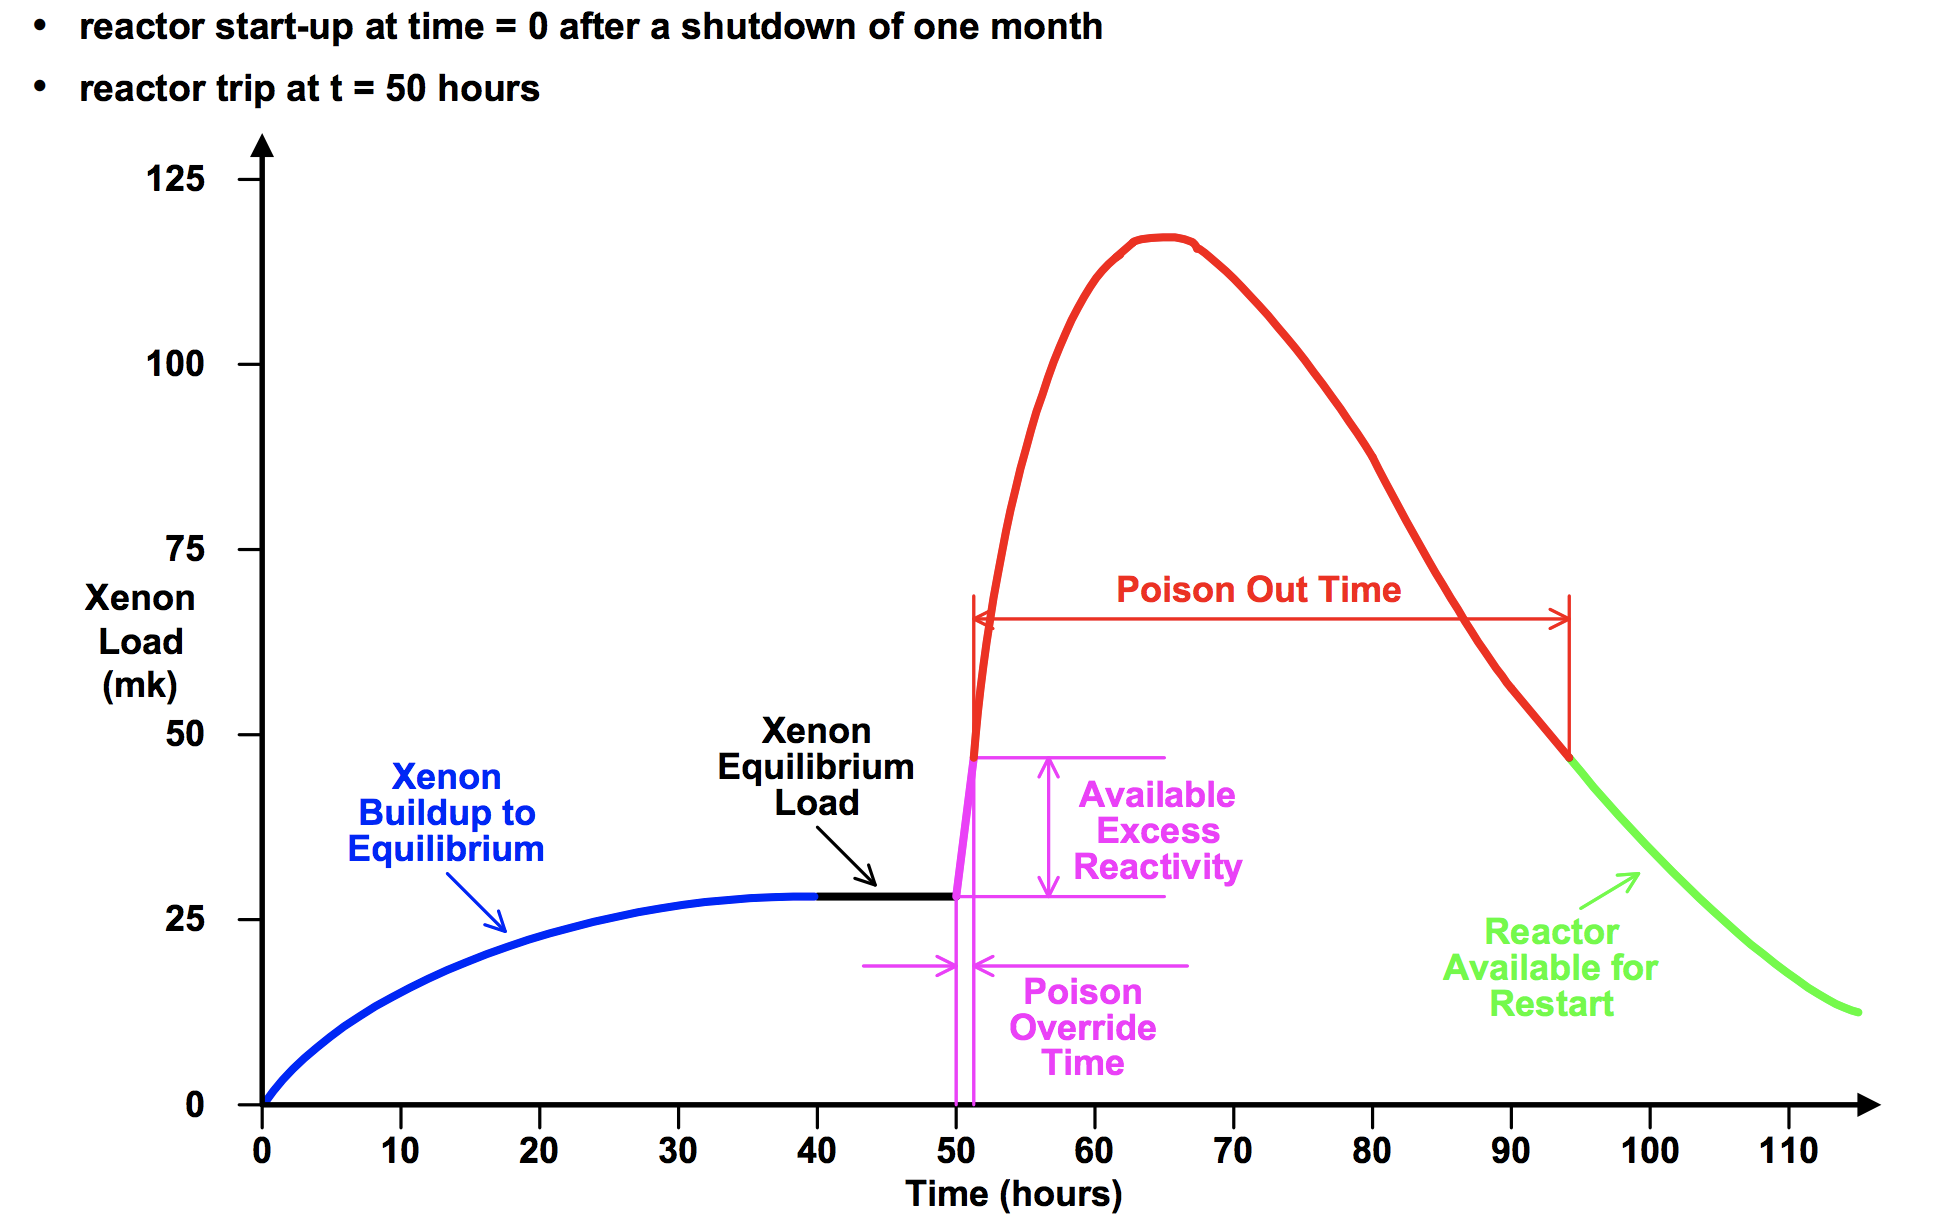
\includegraphics[width=\textwidth]{XenonPoison.png}
\caption{Xenon poisoning effect following shutdown \parencite{garland2005}}
\label{fig:XenonPoison.png}
\end{figure}

Consequently, nuclear reactors aren't well suited to rapid fluctuations in power, particularly dramatic reductions in power, as these can lead to instability in the reactor core.  If the reactor is shut down in order to avoid such dangerous circumstances, it generally cannot be started again until Xenon levels have fallen again, which can take a couple of days.  Obviously this is never desirable for a military vessel, and hence is avoided at almost all costs.

This effect has a dramatic impact on nuclear submarine design, since much of their design is oriented around being able to comfortably disperse large amounts of excess power, rather than with conserving it.  For the propulsion system, this actually makes having an inefficient propulsor at low speeds a considerable advantage.  Since the reactor will likely need to dispose of excess power, particularly during ramp-down, an inefficient propulsion system actually provides a useful power sink.  Since any excess power will have to be disposed of by some other means (normally by pumping more water to remove the power as the heat) inefficiency at low speeds has no penalty, and probably a marginal benefit, since it will reduce overall demand for additional systems.    Provided the excess turbulence inside the pumpjet isn't too noisy, wasting energy through the propulsor is useful.

It should also be noted that a nuclear reactor's aversion to sudden reductions in power would also have a substantial impact on the design of a submarine's combat system, and it's demand on the Hotel Load. For the same reason, a high Hotel Load, or power-hungry Combat System, could actually be advantageous, as it helps to set an elevated 'floor' for power requirements, reducing the scale of fluctuations in overall power demand from the reactor due to changes in propulsion speed.

\section{Some essential concepts}

\subsection{Conservation of Energy}


This is perhaps one of the most fundamental and well-established principals in physics.  The essential idea is that energy can move or change in form, but it isn't ever created or destroyed.  Machines, plants and animals all derive their energy from a particular other source, which can be measured and evalutated to establish the limits of energy available.  Plants collect energy from sunlight falling on their leaves. Humans (as well as combustion engines) capture the chemical potential energy in organic matter, and release it by combining it with oxygen.  Hydro-electric power plants turn the gravitational potential energy of water stored at a height into electricity.

Conservation of energy has a particularly relevant embodiment in fluid flows, which is given it's primary expression in Bernoullis equation.  It says that the total energy in a connected body of fluid is constant, though it can change in form between kinetic energy (movement), gravitational potential energy (it being elevated) the heat energy in the fluid, and the pressure of the fluid.

In different fluids, the dynamics of how energy moves between one and another change.  For example, in gases, heating up a confined piece of gas will increase it's pressure, or if it is unconfined, increase its volume. This is particularly important for understanding gas turbines. In the case of a liquid, however, all the molecules are in close contact, and hence can't increase in volume or pressure substantially except by the creation of steam. As such, in the absence of large amounts of cavitation, the terms in the relationship which are most important for our consideration are the relationships between pressure, and kinetic energy, and gravity.

In the case of most waterjets which propel surface vessels, the water is lifted from the bottom of the hull at the intake to the pump, which is generally incorporated inside the hull. This increase in gravitational potential coincides with a slowing down of the water relative to the vessel-speed. Since the jet in such vessels is generally ejected at the same height as the pump, this potential is never regained, and is technically a loss, however at high speeds such a loss is small relative to the total power ouput.

\subsubsection{Venturi Effect}

In the case of submarines and torpedoes the water doesn't undertake a change in height, since intake and nozzle are generally all in line with the central axis of the submarine or torpedo.  As a consequence, the key relationship in Bernoullis equations is the relationship between the liquids velocity, and its pressure.  The consequence is that when water moves through a pipe (duct, or shroud) it's pressure is inversely related to the square of its velocity.  This means that when a liquid is forced to to travel through a narrowing pipe, it's pressure necessarily decreases as the velocity increases.  This is a simple embodiment of the Venturi effect.

\subsubsection{Flow Diffusion}

The inverse process is where a pipe increases in volume, and the flow is forced to slow down in order to fill the wider area, and the pressure correspondingly increases.  This is a process called 'diffusion', and is important to achieving high pressure levels in many types of water pumps, including those which will be particularly relevant for pumpjets for watercraft propulsion \parencite{hamilton1997}.

\subsubsection{Energy waste and efficiency}
The conservation of energy also has useful implications for how the efficiency of systems is thought about.  In particular, because energy is conserved, identifying inefficiencies in a system necessarily involves identifying where energy goes to doing tasks which aren't useful for the intended purpose.  A perfectly efficient system won't do any work that isn't for the intended purpose.  In the case of analysing the efficiency of propulsion systems, the relevant 'work' is almost always related to moving water backwards to produce thrust.  Moving water in directions other than backwards, including random turbulent flows which wind producing heat rather than thust, are two examples of wasted energy.  Noise in the water also reflects energy which is wasted.

\subsection{Boundary Layer}

When water or any fluid flows with some speed relative to another solid surface nearby, there is some layer adjacent to the surface in which the speed of the fluid is diminished relative to the main flow.  At a microscopic level, there are some molecules of the fluid on the surface which will be effectively static relative to the surface.  The layer of fluid that joins the gap between the static surface, and the part of the flow which is moving at the full flow speed, is called the boundary layer.  Exactly how thick the boundary layer is, and how the fluid moves in the boundary layer, is extremely important for consideration of efficiency of fluid flows over and around solid surfaces.  In particular, a boundary layer can be either turbulent or laminar in nature, and can transition to turbulent flow after a short distnace of laminar flow, as shown in Figure \ref{fig:BoundaryLayer.png}.

\begin{figure}
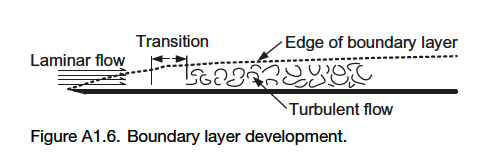
\includegraphics[width=\textwidth]{BoundaryLayer.png}
\caption{The development of a boundary layer \parencite{mollard2011}}
\label{fig:BoundaryLayer.png}
\end{figure}


\subsection{Turbulent and Laminar Flow}

The way that fluids move relative to a surface can one of either two methods.  In 'laminar flow' all the fluid moves in one direction in an smooth and orderly manner, with very little mixing between the layers of fluid travelling at different speeds.

The alternative is 'turbulent flow', where the fluid moves around in unpredictable swirls and circles as well as moving overall in an predominant direction.  There is considerable mixing between all the different layers, and the average speed remains relatively constant in the flow, with the exception of the flow immediately adjacent to the wall, or in the boundary layer.  Becuase turbulence involves a lot of movement that is not overall in one productive direction and contributing to thrust, it necessarily leads to some loss of energy from the overall thrust.  Once the swirls and movements become smaller and smaller, the energy winds up simply as heat in the fluid.


\begin{figure}
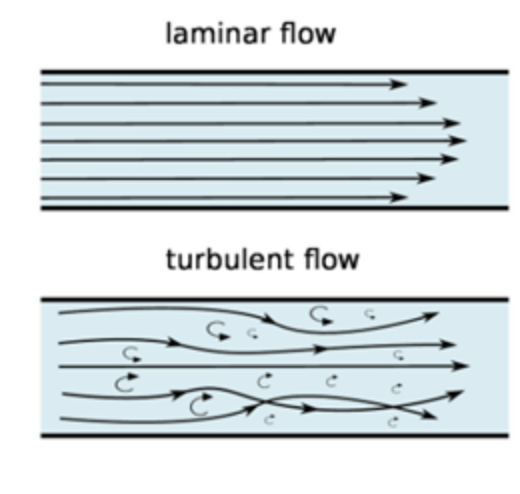
\includegraphics[width=\textwidth]{LaminarTurbulent.png}
\caption{A simple comparison of laminar and turbulent flows from \citetitle{NPdotnet2017} \citeyear{NPdotnet2017}}
\label{fig:LaminarTurbulent.png}
\end{figure}


The likely point of transition between a flow being turbulent and laminar can be given by unitless number called the Reynolds Number, which is determined by a fluids velocity, viscoscity, density, and a characteristic length-scale over which the flow occurring.  A fuller discussion of these important concepts can be found in \citetitle{NPdotnet2017} \citeyear{NPdotnet2017}.

Turbulent flows in gasses can be extremely noisy, since those fluids are compressible.  Consequently, the rapid and intense ciruclar movements result in a lot of oscillatory compressions against the surrounding air.  Consequently things like jet engines, vacuum cleaners, hand-dryers, and other devices that create rapid movements in gasses tend to be quite loud, including at some distance.

In essentially incompressible fluids, the random changes in pressure and velocity which are involved in laminar flow tend not to generate nearly as much noise in the surrounding liquid outside the flow.  Because the fluid is incompressible, all of the random 'round and round' movements don't amount to much 'in and out' movement, which is what creates the pressure waves which result in propagated noise. Consequently, whilst turbulent flows do inevitably generate some noise, the amount of noise generated is dramatically greater in the presence of cavitation, where a void opens up in the water, and vastly more 'in and out' movement is able to occur.

\subsection{Cavitation}

Cavitation is the rapid expansion and collapse of a void, or bubble in water. Put technically, caviation occurs when the local static pressure (pressure in the rest frame of the fluid) falls below the vapour pressure of the fluid (pressure at which the liquid will start to boil).

Imagine what happens when something moves very fast through water.  The front side of the object pushes the water forward, but on the back side the water has to push in to fill the space left behind.  If there’s not enough pressure to push the solid water in fast enough, a gap opens up, with just a few gaseous water molecules (steam) inside the cavity.  (This is also described as water boiling at low pressure.)  However the gap doesn’t stay around for long.  Soon the water catches up, and the bubble implodes with a pop, leaving only tiny bubbles as a result, which you can see in the wake of almost any boat or ship moving at speed.  Whilst some energy turns to heat (the remaining steam in the tiny bubbles) quite a bit is propagated away as a sound-wave generated by the implosion.

A watching water boil in a glass kettle gives a quick and intuitive insight into the occurrence of cavitation.  Quickly after the kettle starts heating, a considerable noise can be heard, which corresponds to the commencement of cavitation on heating element. At some local point for a moment in time, there is enough energy for the water present to boil.  It tends to be on rough surfaces or in the presence of some impurity that cavitation will occur first (in the blackened part of the surface in this case.)  However, whilst the bubbles on the bottom can be seen plainly on the bottom, they collapse almost straight away again, and leave only a tiny bubble of stable steam ciculating in the water.  It is the rapid expansion and collapse of these bubbles that causes the noise of a kettle, long before it has boiled.

\begin{figure}

\includegraphics[width=\textwidth]{EarlyCavitation.JPG}
\caption{Cavitation bubbles form and collapse creating noise and some tiny bubbles long before boiling occurs}
\label{fig:EarlyCavitation.JPG}
\end{figure}

It is only when the water is all at a much higher temperature that the bubbles remain their full size for long enough to detatch and rise all the way to the surface, a process we typically think of as boiling water, as shown in Figure ~\ref{fig:BoilingCavitation.JPG}.  It is worthwhile noting that the sound emitted at this stage is much softer and lower than the early onset of cavitation. Larger bubbles result in lower frequencies of sound being emitted. Even at higher temperature, the rougher parts of the surface provide the points where all the cavitation originate.

\begin{figure}

\includegraphics[width=\textwidth]{BoilingCavitation.JPG}
\caption{Only at very high temperatures do the bubbles endure at full-size in the water and reach the surface}
\label{fig:BoilingCavitation.JPG}
\end{figure}


Cavitation is extremely important in the study of ship propulsion, since it's occurrence in particular circumstances can lead to substantial losses of efficiency, as well as damage to the propeller and related appendages. It is particularly important for submarines, since the expansion and collapse of these bubbles tends to lead to the creation of noise which is often far larger, and more distincly characteristic than other turbulent disturbences in the water when no cavitation is present.  Consequently, the onset of cavitation can be thought of as a distinct threshold in terms of the acoustic performance of propulsive system.

Despite cavitation necessarily representing some energy being wasted generating unwanted noise in the water, some cavitation inevitably occurs around most propulsion systems operating at full power.  In plenty of cases, the consequences for efficiency are relatively small, as they tend to be dominated by other efficiency considerations in imparting thrust.  Put another way, the savings that can be gained by minimising wastage to turblence can outweigh the losses incurred by having some cavitation occur.  In most cases, propellers are designed to work with a certain extent of cavitation for optimum efficiency under working loads \parencite{shin2015}. Cavitation also occurs to a considerable extent within the jets of most high-speed surface vessels, but doesn't necessarily have a particularly bad effect on their overall efficiency at their intended speed levels.  It is generally only within very specialised military circumstances when the absolute avoidance of cavitation supercedes other concerns for efficiency, and require the elimination of all cavitation entirely \parencite{mollard2011}, \parencite{lewis1988}.  These circumstances include the design of submarines and torpedoes.

In certain special cases, particularly supercavitating propellers or surface-piercing drives, high levels of cavitation can be higly advantageous for efficiency.  However these represent specialised designs, generally only for very high speed vessels, where acoustic concerns are negligible, and are of little concern for this particular endeavour.

Cavitation can occur in a number of different ways at different points and forms on or around the propeller.  It is common for cavitation to occur first near the out extremities of the propeller, where the blades are moving at the highest velocity relative to the water-flow.  Cavitation tends to spread across the back of the blades in a sheet (sheet cavitation), since the back side of the blades are generally the areas of most depressed pressure, though it can also occur in places on the back side of the blades, where the dynamics of the water moving around the blade can produce points of near the edges of significantly reduced pressure. On surface vessels cavitation tends to occur most when the blades are closes to the surface, where the pressure is lowest.


\begin{figure}
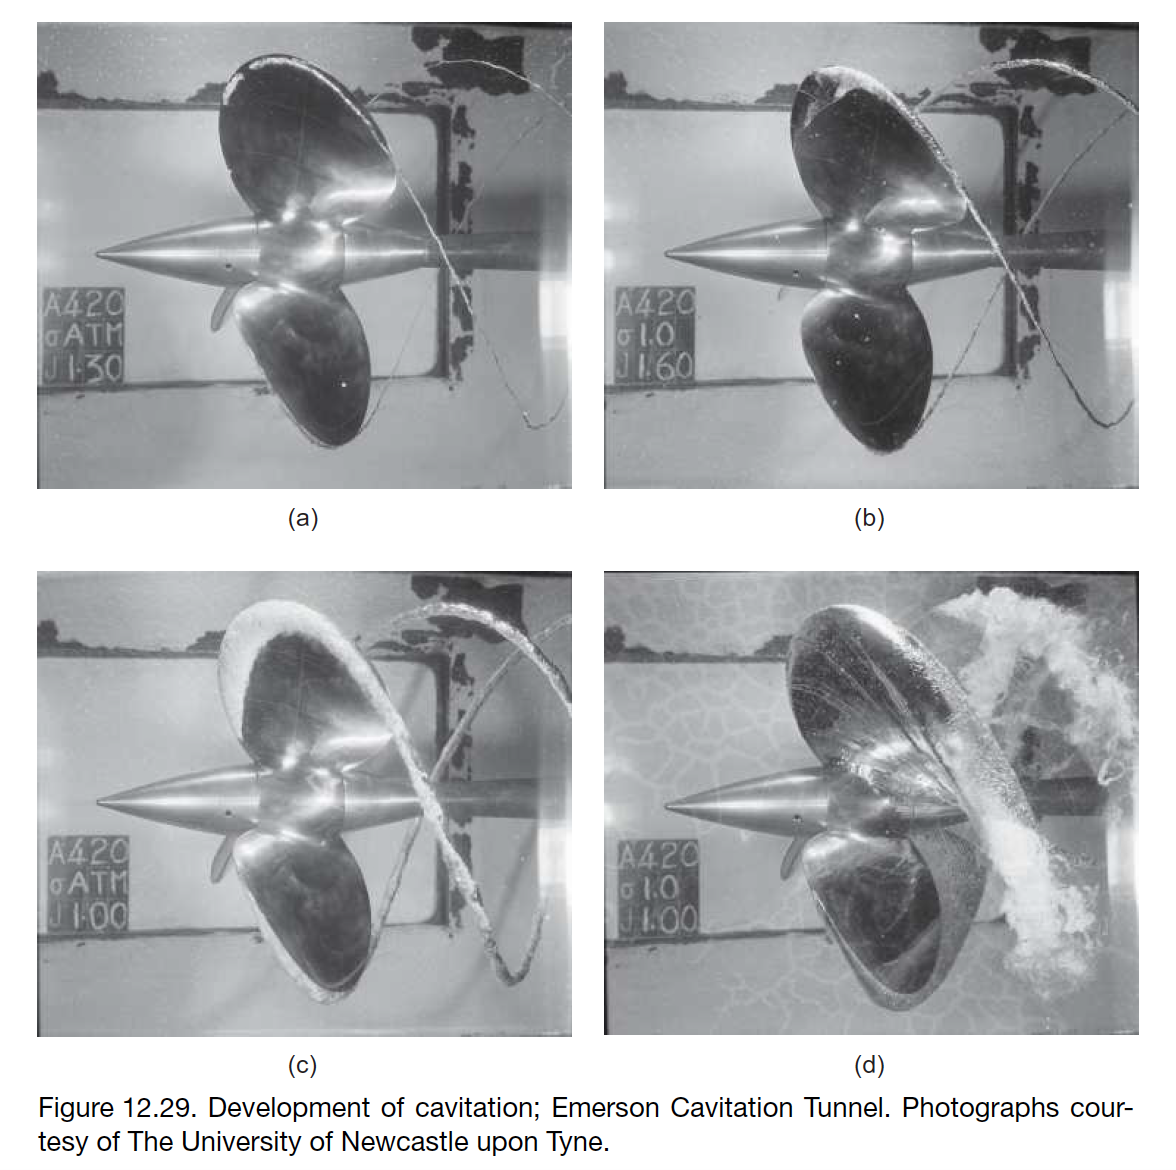
\includegraphics[width=0.7\textwidth]{IncreasingCavitation.png}
\caption{Cavitation frequently occurs first at the extremities, then spreads inwards across the blad face, as shown in \parencite{mollard2011}}
\label{fig:IncreasingCavitation.png}
\end{figure}


\begin{figure}
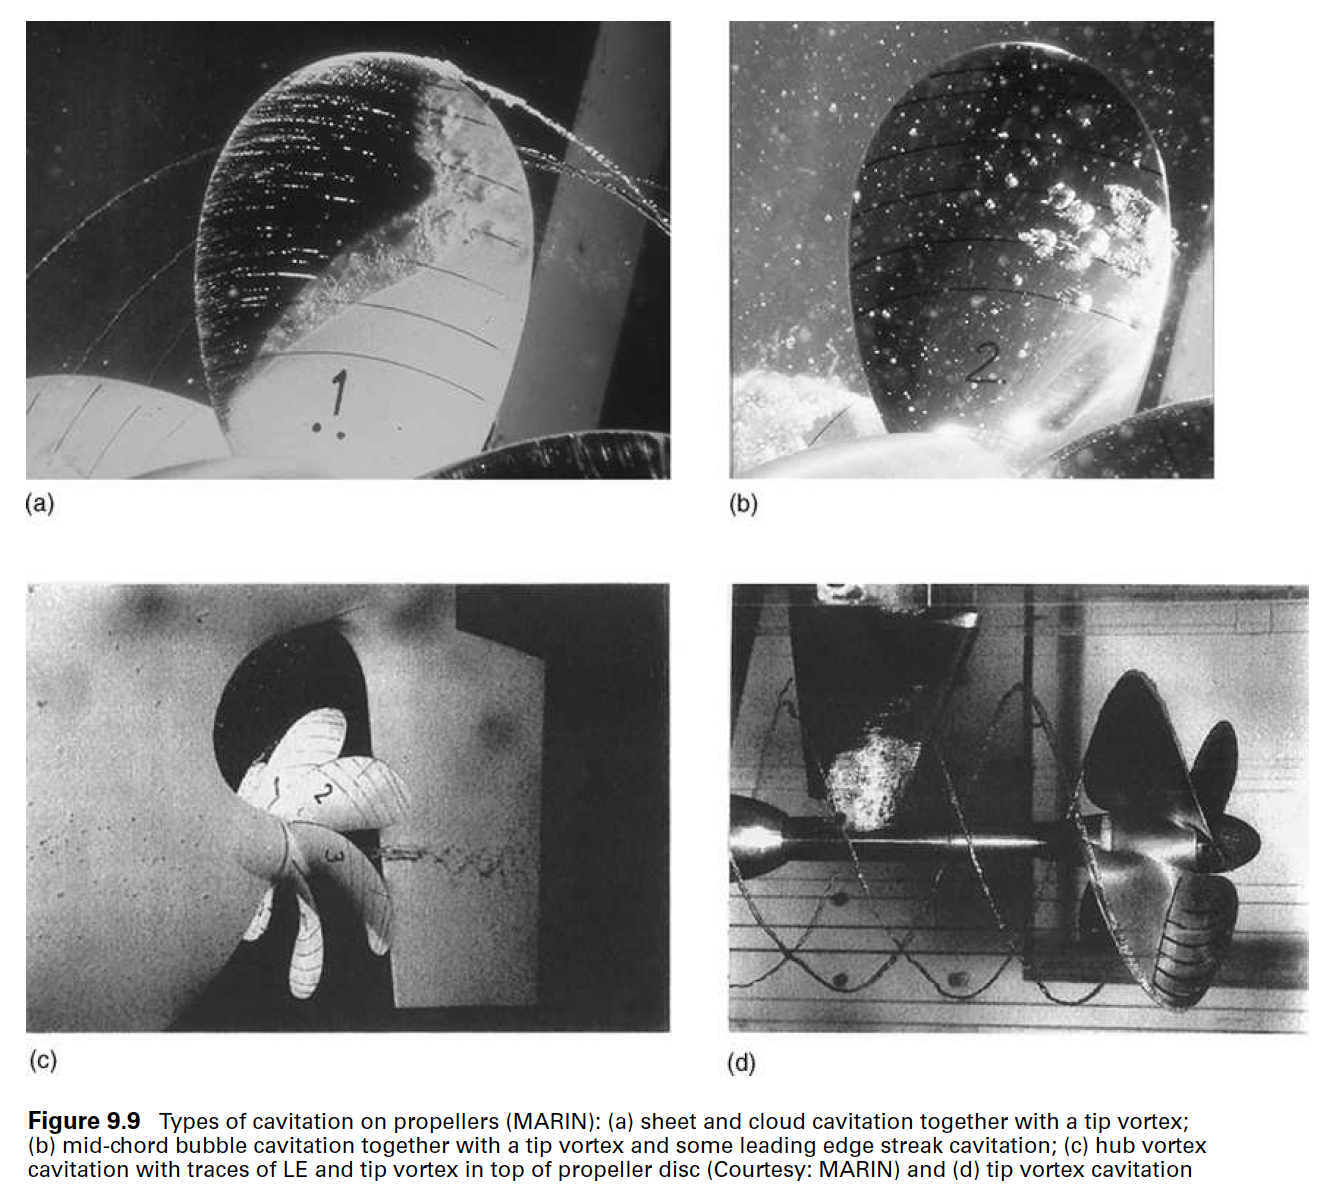
\includegraphics[width=0.7\textwidth]{CavitationTypes.png}
\caption{Different types of cavitation can occur on different parts of the propulsion system as shown in \parencite{carlton2007}}
\label{fig:CavitationTypes.png}
\end{figure}

\subsection{Pressure, Thrust, and Momentum change}

It is worthwhile spending just a moment to touch on the relationship between a few different concepts which are closely related.  Thrust is a force, measured in Newtons, which is generally used to refer to the forces acting on a vessel or object by its propulsion system to move it forward in the water.  Generating thrust is consequently a key objective of any propulsion system.

Pressure is a measure of force divided by an area over which it is applied. Pressures are necessarily applied to some extent over all of the surfaces of any object, including due to the atmostpheric pressure of air.  In considering the efficiency of propulsion systems for solid bodies, thrust is always the consequence of some \textbf{net} pressure difference on different sides of an object.  For instance, on a propeller blade, the rear-facing side of the blade is the side that pushes the water backwards, and hence has a raised pressure on its surface.  Being generally backwards facing this acts to push the propeller forwards.  This pressure acts equally to push water backwards, as well as to push the propeller forwards.  Importantly, the forward-facing side of the propeller will expereince a lowered pressure, which also serves to pull water backwards, and suck the propeller forwards.  It is the sum of all the pressure differences on the propeller that result in a net force.

Importantly in hydrodynamics, it is important to consider the possibility of other forces being generated other surfaces which may have an impact on the movement of the vessel.  In the presence of the hull, water being drawn by the propeller can cause pressure changes on other surface of the vessel which may assist or impede producing a net positive thrust.  Submerged jets represent a particular case in point.  A famous home experiment suggests that one compare the thrust (backwards pressure) experienced by someone holding a garden hose creating a jet of water when it is in the air, as opposed to submerged in a pool of water.  When submerged, the backwards pressue appears dramatically reduced.  In fact, this phenomenon is due to a the water-jet drawing adjacent water with it under-water, the movement of which exerts a negative pressure on the outside of the nozzle, conteracting the pressure exerted on the inside of the nozzle. This effect represents one of the important distinctions between the jets which release their water below or above the water-line.

It is also an important law of physics that force or thrust is equal to the rate of change of momentum. Put simply, the speed at which one speeds something up, or the increasing amount of something which begins to move, is always equivalent in magnitude to the thrust that is produced.  Since momentum is a vector, this simple law requires that the momentum change has to net out to one particular direction in order to produce a net thrust.  Circular movements necessarily are cancelling, and produce no thrust. It is useful to recall however that this principal is simply another complete and way of measuring the consequences of the net pressure differences discussed earlier.  The total rate of change of momentum in the water-column which is induced as a conseqence of the pressure differentials on all sides of the propeller must necessarily be equivalent to the total net force that is produced.  Consequently literature seeking to optimise propulsion might discuss analysis referring to both of these effects or phenomena, and neither are in conflict.

Full and proper derivations of many of the thrust equations for different propulsion systems from these principals can be found in plenty of authoritative works, including \parencite{lewis1988}, \parencite{carlton2007} and \parencite{mollard2011}.

\subsection{Flow separation}

Flow separation refers to a circumstance when the flow over a surface separates entirely from the surface, and a new eddy or votex is formed where the flow actually moves in the opposite direction to the dominant flow.  It is of particular significance in hydrodynamics because it can lead to substantial losses of efficiency, as energy is diverted into the kinetic energy of the eddy or vortex, which is unproductive. It tends to occur near the surface of aerofoils with high angles of attack, or in the blades of turbomachinery including diffuser or mixed-flow pumps and ducted propellers operating in off-design conditions, including low flow rates \parencite{li2013}  \parencite{bakker2006} \parencite{mcbride1979} \parencite{wislicenus1986}.

\begin{figure}
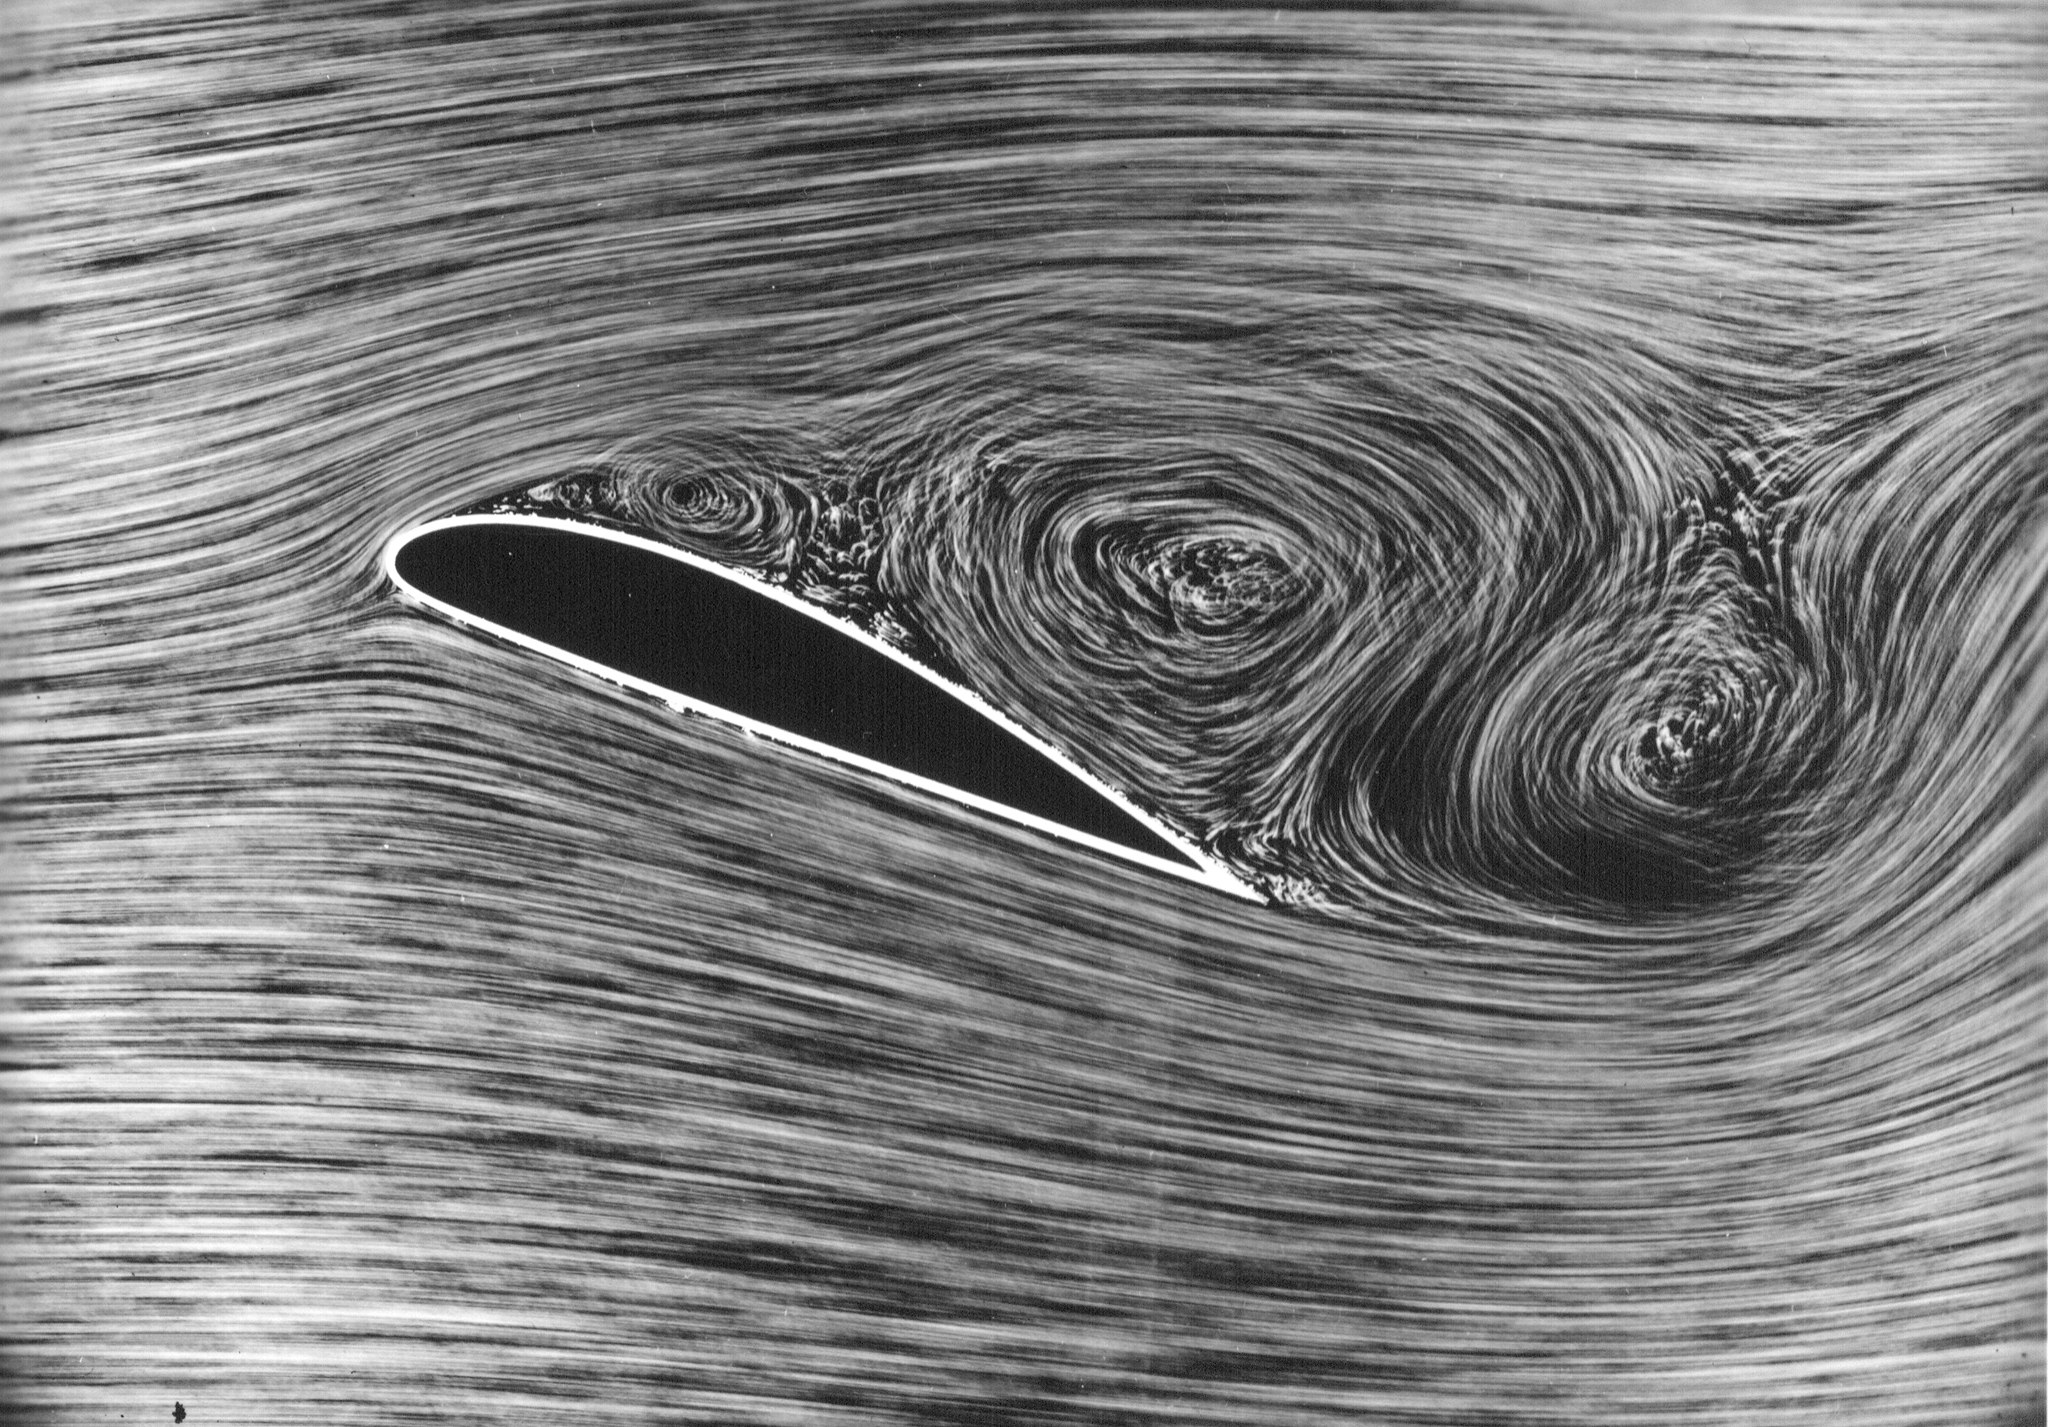
\includegraphics[width=\textwidth]{SeparatedAerofoil.jpg}
\caption{Flow separation occurring over the top of an aerofoil in a wind tunnel. Image courtesy of Deutsches Zentrum fuer Luft- und Raumfahrt e. V. (DLR)}
\label{fig:SeparatedAerofoil.jpg}
\end{figure}

In order for flow separation to occur, a fluid must be moving against an adverse pressure gradient, which simply means that the pressure is increasing in the direction of movement, which means the flow is slowing down as it moves.  At the boundary layer, where the flow velocity is already reduced due to drag forces experienced near the surface, the adverse pressure gradient can be enough to reverse the flow altogether.  In this case, the fluid flows in reverse near the surface and forms a vortex, and the main flow becomes separated form the surface by the votex.

\begin{figure}
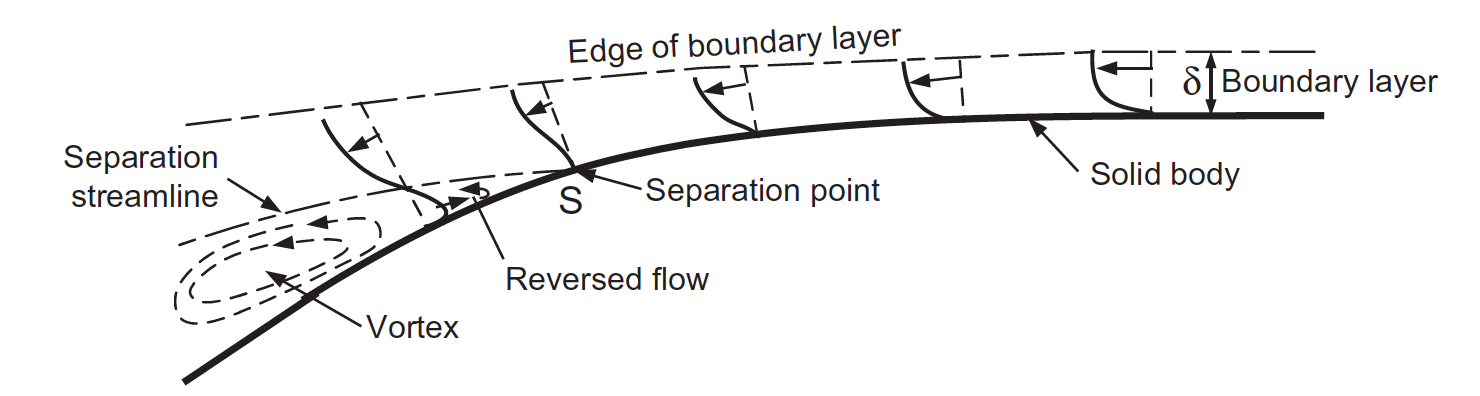
\includegraphics[width=\textwidth]{FlowSeparation.png}
\caption{Flow separation involves flow reversal near a surface when a fluid is moving against an adverse pressure gradient, as shown in \parencite{mollard2011}}
\label{fig:FlowSeparation.png}
\end{figure}

In addition to the necessary loss of efficiency, flow separation can often tend to result in unsteady flows, with the vortices periodically being shed into the flow [@mollard2011 pp. 480].  If this occurs ahead of the blades of a propeller or impeller, such disturbances to the flow can lead to instances of cavitation when otherwise a steady homogenous flow might be well below the cavitation inception point, and can be consequential for the acoustic performance of the system, particulaly if such shedding resonates with characteristic frequencies of any of the machinery.

\section{Basics of Ducted Propellers and Pumpjets}

It's easy to be somewhat confused by the many different names which seem to be associated with related, or similar systems.  Between pumps, pumpjets, water-jets ducted or shrouded propellers, or impellers, there is plenty of grounds for some confusion  In this section, I aim to clarify in simple terms what the important differences between distinctly different systems are, and where some terms are used somewhat interchangeably without doing any great violence to the concepts underlying.

\subsection{Propellers}

Perhaps the best starting point is the most basic, and oldest of the systems which we're considering: the basic screw propeller.  A propeller uses a number of tilted blades attached to a central hub to sweep around disc in the water, and accelerate a column of water passing through the disc.  Due to the slant of the blades, water on the back sides of the blades is pushed astern, and reduced pressure on the front faces pulls more water from ahead to replace it.  As such, it accelerates a column of water, which necessarily is contracted in circumference after the point of acceleration.

\begin{figure}
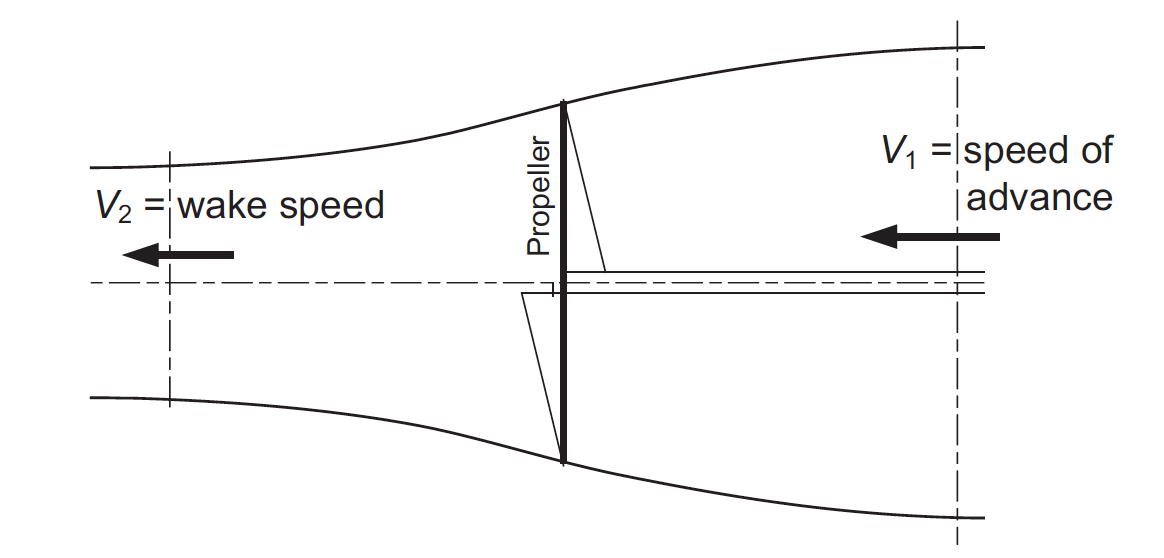
\includegraphics[width=\textwidth]{PropellerAction.png}
\caption{Propellers generate thrust by accelerating a column of water, as shown in \parencite{mollard2011} page 247.}
\label{fig:PropellerAction.png}
\end{figure}

A comprehensive description of the development of the propeller can be found in \parencite{@carlton2007}.  Here I won't elaborate on beyond describing some essential features and characteristics with which one ought to be familiar, primarily for the purpose of comparing different propellers and their evolution into impellers of different designs.

Most propellers will have between three and seven blades.  In general they are shaped as an aerofoil, with the convex side being upstream, just as the convex side of a plane wing is above, in order to generate lower pressure and lift as it moves through the air.  The blades tend to be twised so that they have a higher angle of attack closer to the hub, and lesser closer to the extremities, so that those faster moving sections push their respective parts of the water column at an overall similar speed.  The are often also thinner towards the extremities, and will be swept backwards as if dragged by their rotation through the water (skew) and also dragged by the ship's movement throug the water (rake), as seen in Figure ~\ref{fig:SkewRake.png}. Whilst the degree of all these characteristics is highly variable for different applications, these are a few of the commonly referred to characteristics which can be varied in order to optimise performance for any given application.

\begin{figure}
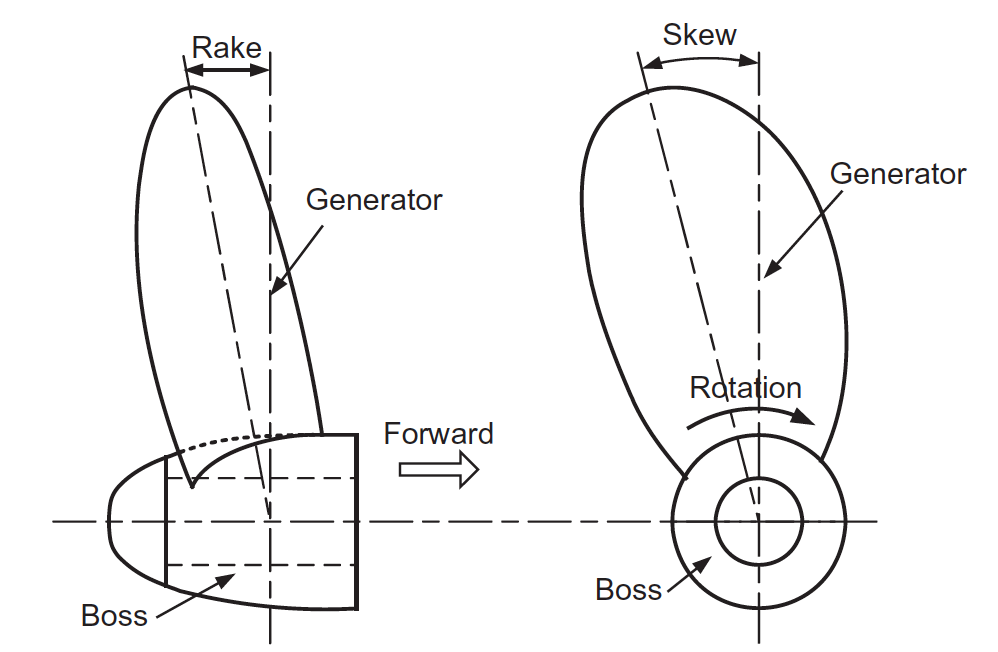
\includegraphics[width=\textwidth]{SkewRake.png}
\caption{Propeller geometry including skew and rake, as shown in as shown in \parencite{mollard2011} page 262.}
\label{fig:SkewRake.png}
\end{figure}

\subsubsection{Pitch}
Perhaps one of the most important characteristics of a propeller is its pitch.  The pitch represents the distance that a blade section would travel forward if it carved its way around a helix through one full rotation.  It is intuitive to think of as something akin to the angle-of-attack of the propeller blade to the water, however this is technically misleading as the movement of the water-column incoming to the blade, as well as the speed of rotation, also have a significant bearing on what the actual angle of attack of the blade ends up being.  Whilst technically pitch is a distance (measured in meters), it is often expressed and used in formula as a ratio of the diameter of the propeller, to give it a unitless equivalent, as is common in the description of propellers and propulsion systems.

\begin{figure}
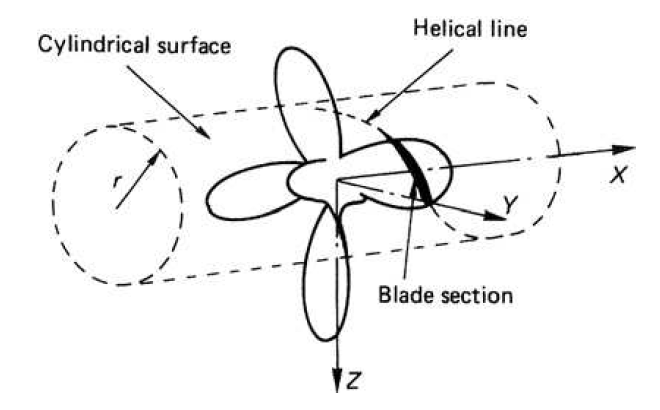
\includegraphics[width=\textwidth]{HelicalLine.png}
\caption{A blade section of a propeller traces a helical line around a cylinder as it is rotated as shown in \parencite{carlton2007}}
\label{fig:HelicalLine.png}
\end{figure}

\begin{figure}
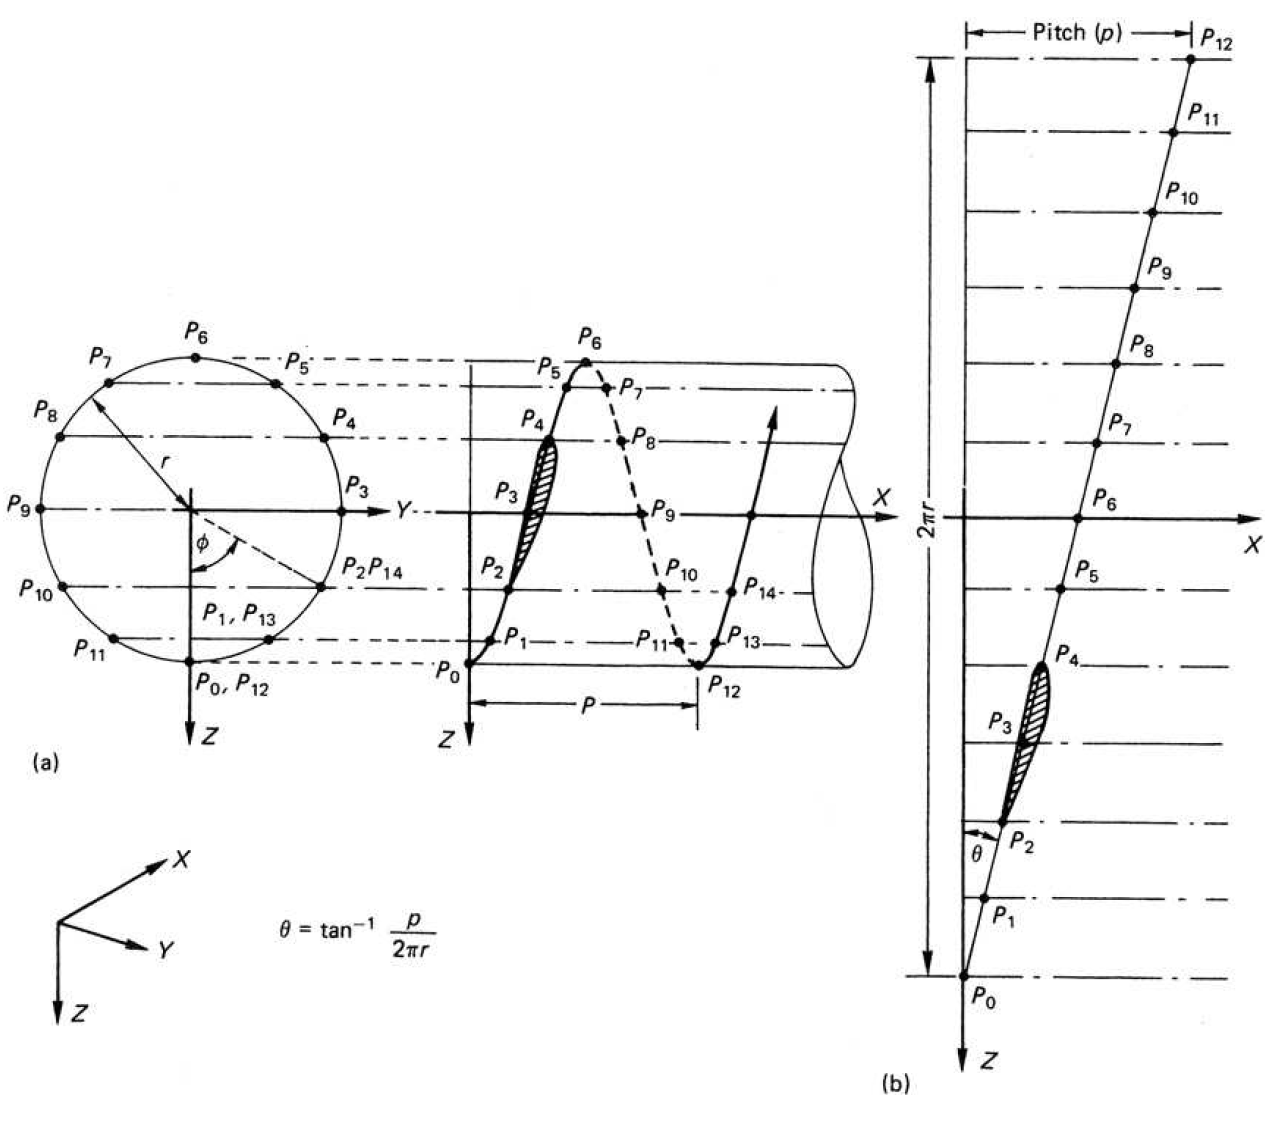
\includegraphics[width=\textwidth]{PitchDefinition.png}
\caption{The definition of pitch is the distance traveled by a blade section along a cylinder, as shown in \parencite{carlton2007}}
\label{fig:PitchDefinition.png}
\end{figure}

The selection of the exact blade selection that is selected to define pitch must be specified as being at some fraction of the radius from the centre.  This distance is calculated to be the 'moment mean' or a technical derived effective average, which tends to lie between 0.6R and 0.7R.  A thorough discussion of pitch can be found in \parencite{carlton2007} pages 35-37.

Pitch is of particular importance to the discussion the efficiency of propeller and propulsor design because its optimal choice tends to vary considerably with the different loads which a vessel is intended to operate at, which can also relate to a vessel's design speed.  It is for this reason that a considerable number of vessels actually have variable pitch propellers.  Whilst considerably more complex, expensive, and heavier than a traditional fixed-pitch propeller, the ability to vary the pitch of a propeller assists considerably, particularly when the amount of load (resistance) a vessel is expected to face varies considerably.  Controllable pitch propellers also have advangates in terms of manouverability, since the pitch can be reversed and hence reverse thrust can be produced, without requiring the direction of the power coming from the engines to be reversed.  This has advantages for ferries which undertake frequent docking manouvres in confined spaces \parencite{MAN2017} \parencite{lewis1988}.




In Figure \ref{fig:ex2} we can see a sample plot of the mtcars data.

\begin{figure}
\begin{knitrout}
\definecolor{shadecolor}{rgb}{0.969, 0.969, 0.969}\color{fgcolor}

{\centering 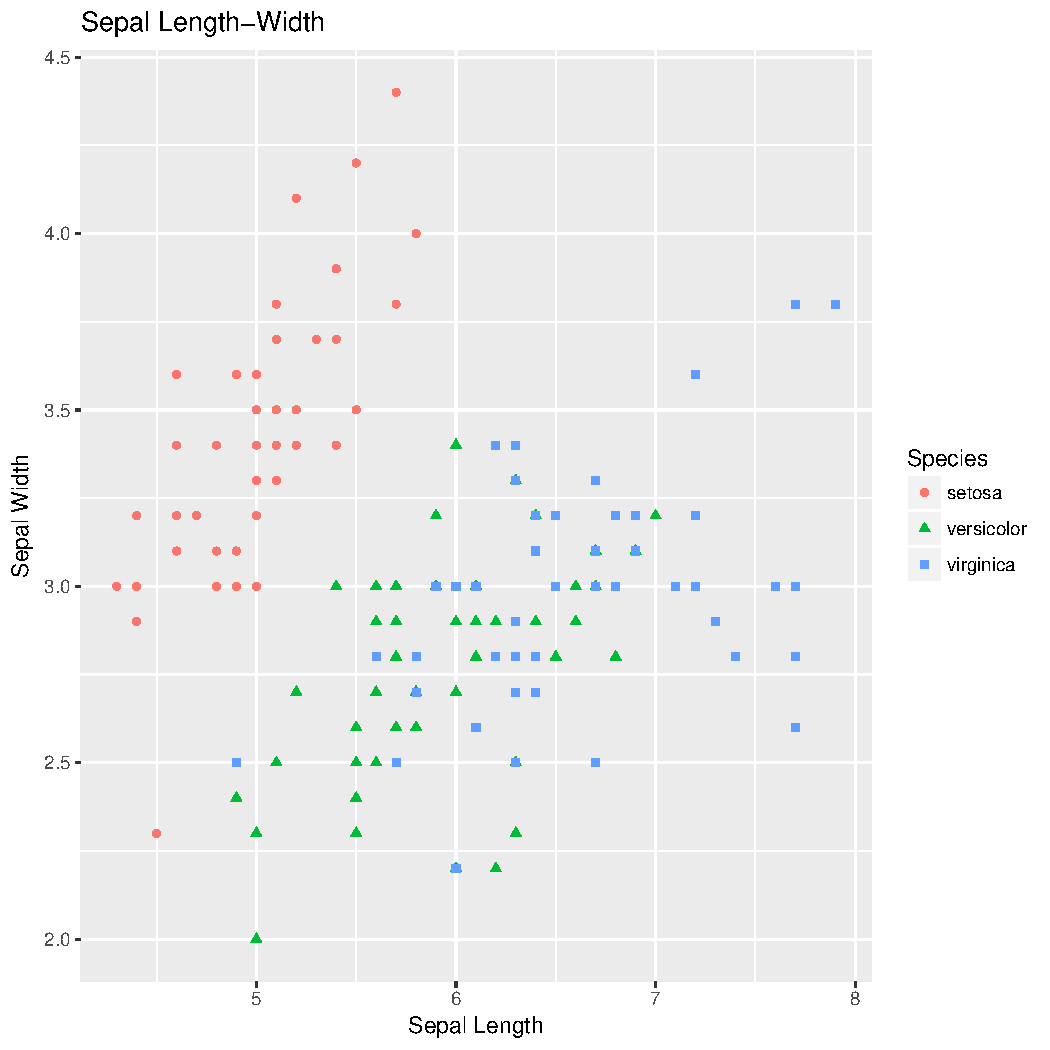
\includegraphics[width=\maxwidth]{figures/plots-unnamed-chunk-1-1} 

}



\end{knitrout}
\caption{An example plot}
\label{fig:ex2}
\end{figure}




\printbibliography

\end{document}
